% Meta-info: Java version, build environment, RMI
\subsection{Environment}
\paragraph{}{
    To build the Gcom project, you need a working distribution of maven, java
 1.7 or above. Some scripts are available in the \texttt{bin} folder, assuming
 you use bash.
}


% Building JAR
\subsection{Compiling Gcom}
\paragraph{}{
    To use the Gcom artifact, you need to compile and package it. To do so,
 just run \texttt{mvn package} in the Gcom folder. The sub-directory
 \texttt{target} may now contain two jar files, \texttt{Gcom-4.2.jar} and
 \texttt{Gcom-4.2-jar-with-dependencies.jar}. The first one can be imported
 to a new project and can be used as a library. The second jar file is the 
 project packed with all needed dependencies and can be use to run directly
 the name server needed by Gcom.
}

% Starting nameserver
\subsection{Name Server}
\paragraph{}{
    To run the name server simply run \texttt{nameserver.sh} in the
 \texttt{bin} folder. Then the name server should run. You can recompile
 and repack the program by adding \texttt{compile} to the program
 arguments. Another way to run the name server is to run the jar file
 using \texttt{java -jar target/Gcom-4.2-jar-with-dependencies.jar},
 assuming the working directory is the \texttt{Gcom} folder.
}

% Demo chat-app description
\subsection{Gchat, the toy demo of Gcom}
\paragraph{}{
    To show off and prove Gcom works, we build a demonstration application,
 Gchat. It is basically a chat build on top of Gcom.
}

\begin{figure}[h]
    \begin{center}
        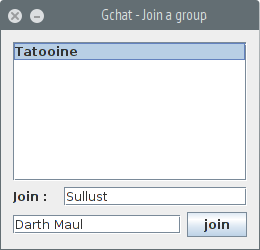
\includegraphics[scale=0.6]{figures/gchat_connection.png}
    \end{center}
    \caption{Connection window of Gchat}
    \label{fig:gchat_connect}
\end{figure}

\paragraph{}{
    The application can be found in the sub-directory \texttt{Gchat}. 
 A script in the \texttt{bin} directory allow you to run the application easily
 by running \texttt{chat.sh}. The script need in the same order : a multicast 
 strategy, that defines the way the communication module will send messages to
 the other nodes, a ordering, that define the way messages will be processed and
 the host name (or the IP address) where the name server runs. \newline
 There are three different multicast strategies, the tree base (\texttt{tree}),
 which is not stable, the unreliable multicast (\texttt{unreliable}) and the
 reliable one (\texttt{reliable}). \newline
 As well, there are three different ordering ways, \texttt{fifo}, which is the
 first in, first out way and need to be more tested. \texttt{causal} order and
 the \texttt{unordered} strategies. \newline
 If need, the application can be (re)compiled by giving \texttt{compile} as an
 argument of the application. Finally you can run the debug mode by adding 
 \texttt{debug} to the arguments.
}

\begin{figure}[h]
    \begin{center}
        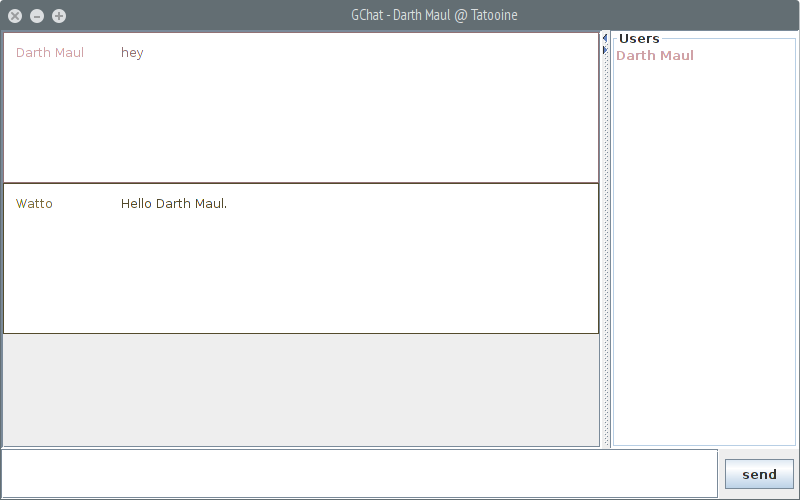
\includegraphics[scale=0.4]{figures/gchat_chat.png}
    \end{center}
    \caption{Chat window of Gchat}
    \label{fig:gchat_chat}
\end{figure}

% Starting client and creating or joining group
\paragraph{}{
    Figures \ref{fig:gchat_connect}, \ref{fig:gchat_chat} and \ref{fig:debug_gui}
 present the connection window of the chat, the chat window and the debug GUI
 which is a part of the Gcom module. \newline
 The connection window allow the user to choose an existing group or to join
 a new one by editing the name of the group in the input area. The user can also
 choose a different name by editing the name randomly chosen. Finally, the user
 can join a group by click to the join button. \newline
 Once the user joined a group, he is able to send messages and receive messages
 from the group. A list of the users which are in the group are displayed
 on the right.
}

\begin{figure}[h]
    \begin{center}
        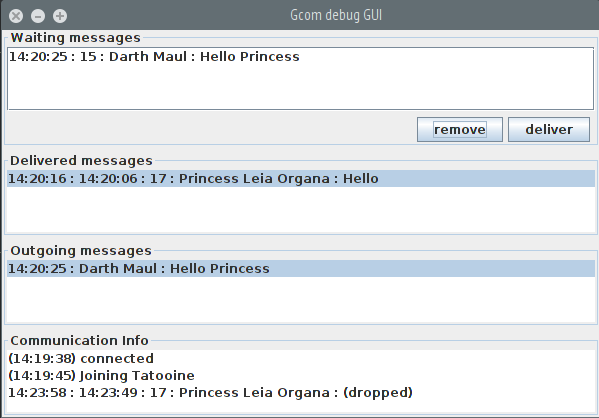
\includegraphics[scale=0.5]{figures/debug_window.png}
    \end{center}
    \caption{Debug interface of Gcom}
    \label{fig:debug_gui}
\end{figure}

\paragraph{}{
    The debug interface is divided in four list which display messages
 regarding what happen into the Gcom module. As we can see on the figure
 \ref{fig:debug_gui}, the top list displays the messages we get from
 the network. Two buttons remove and deliver can be use to
 respectively drop a message or deliver it to the ordering module.
 When a message is delivered to the ordering module, it is processed
 and it should appear into the Delivered messages list. \newline
 All messages send by the user are displayed in the Outgoing messages
 list. Finally, the last list, communication information display
 several type of messages, as when the chat is connected to the
 nameserver, when the user join a group, which messages are
 dropped, and so on. The list display the messages send and received
 by the communication layer of Gcom. \newline
 Each messages are displayed with the local time when they are
 received.
}

% trouble shooting ?
\subsection{Trouble shooting}
\paragraph{}{
    The main problem you can get may concern the name server.
 If you get message telling the application can't connect to the
 name server you might mispell the IP address or the host name
 where the name server runs, or, you may start (or restart) the
 name server if you don't already start it. \newline
 You may also get an error telling the name server can't be start,
 it may arrived in two cases : a name server if already running
 or the port used by Gcom is already used another application.
}


% Further dev
	% Create own application using Gcom

